% Created 2021-12-27 Mon 22:17
% Intended LaTeX compiler: xelatex
\documentclass[a4paper]{apa6}
\usepackage{graphicx}
\usepackage{longtable}
\usepackage{wrapfig}
\usepackage{rotating}
\usepackage[normalem]{ulem}
\usepackage{amsmath}
\usepackage{amssymb}
\usepackage{capt-of}
\usepackage{hyperref}
\threeauthors{杨润泽 ZY2106227}{蒋宇聪 SY2106217}{罗哲焱 SY2106118}
\threeaffiliations{北京航空航天大学}{北京航空航天大学}{北京航空航天大学}
\leftheader{数据分析中的结构信息原理}
\shorttitle{结构信息}
\usepackage{ctex}
\usepackage{breakcites}
\usepackage{apacite}
\usepackage{natbib}
\usepackage{paralist}
\usepackage{bm}
\let\itemize\compactitem
\let\description\compactdesc
\let\enumerate\compactenum
\abstract{本次作业介绍了结构信息论的基本知识:图的编码方法以及编码树的概念,由给定的编码树所确定的图结构信息,进而引出图结构信息熵的定义。在介绍了图结构熵极小化算法后对图结构信息论在多个实际问题上的应用进行了讨论,包括图结构熵解码低分辨率Hi-C数据的染色质拓扑结构域方法,以及基于结构信息的文本聚类和基于结构信息的局部列举排名算法。}
\keywords{结构信息,拓扑结构域,文本聚类}
\date{\today}
\title{计算理论大作业--数据分析中的结构信息原理}
\hypersetup{
 pdfauthor={Justin},
 pdftitle={计算理论大作业--数据分析中的结构信息原理},
 pdfkeywords={},
 pdfsubject={},
 pdfcreator={Emacs 27.2 (Org mode 9.5)}, 
 pdflang={English}}
\begin{document}

\maketitle

\section{引言}
\label{sec:orgbb1ae0d}
21 世纪出现了网络数据、生物数据、医学数据等新型数据,这些大数据是本世纪一个新的科学现象,是经典数学概念在信息时代的表现形式,但又实质性地区别于经典数学。简单地说,大数据是由规律嵌入在噪音中形成,信息处理的任务就是在大数据中区分出规律与噪音。现有信息科学与工程的核心工具是香农创立的信息论。香农在 1948 年给出了一个概率分布的信息度量, 即信息熵。对 于一个概率分布 \(\boldsymbol{p}=\left(p_{1}, p_{2}, \cdots, p_{n}\right)\), 满足 \(\sum_{i=1}^{n} p_{i}=1, \boldsymbol{p}\) 的熵 \(H(\boldsymbol{p})\) 定义为:
$$
H(\boldsymbol{p})=-\sum_{i=1}^{n} p_{i} \cdot \log _{2} p_{i} .
$$
准确地说, \(H(\boldsymbol{p})\) 是一个数, 它度量了一个概率分布 \(\boldsymbol{p}=\left(p_{1}, p_{2}, \cdots, p_{n}\right)\) 的不 确定性, 这里不确定性是指信息, 而熵或信息量是不确定性的度量, 是一个数。对概率分布而言,熵和信息可以不做准确的区分,两者类似于力和反作用力,大 小相等,方向相反。举个通俗易懂的例子,如一支足球强队和一支足球弱队进行 足球比赛,赛前谁赢是不确定的,不确定性就是熵,比赛结束后得到一个信息, 所得到的信息量就是赛前的熵。按照实力来讲,强队获胜的不确定性很小,那么 熵就小,赛后强队取胜,那么观众得到的信息量就少;相反,弱队获胜的不确定 性非常大,获胜概率很小,那么熵就大,赛后如果弱队取胜,那么观众得到的信 息量就非常多。因此熵是事前不确定性的量,信息是事后所得到的信息量,即消除的不确定性。

香农熵实质是一个概率分布不确定性的数学度量。然而概率分布是没有结构的,但大数据的实质是数据之间存在关联关系,因此研究概率分布的香浓信息论不足以支撑大数据分析。利用信息的结构理论支持网络分析是计算机科学的一个重大挑战。有很多方法把图去结构变成无结构的概率分布,然后应用香农熵来定义 图的信息。当从一个图 G 中提取分布 p 时就丢失了 G 的结构, 而对于很多系统(例如图),其结构是实质性的,真正有意义的信息是嵌入在系 统结构中的信息,它决定并解码出该系统的一个实质结构,而这个实质结构支 撑着复原原系统的功能语义。因此把图转换为概率分布的方法都不能很好地给出一个信息的结构 理论以支持网络分析。Li 和 Pan\citep{li_structural_2016}在 2016 年提出图的树编码方法、图结构熵的 概念,第一次提出了一个结构信息的度量,并进行了理论证明,建立起了结构信 息论的基本框架。结构信息论\citep{li_structural_2016}是刻画图结构信息这一重大科学问题的原始创 新成果。结构信息论的核心概念是结构熵。直观来说,结构熵是定义在一个图上 的用于刻画图结构不确定性的基本度量。结构熵定义的核心思想是图结构可以 通过其上的一个随机游走过程来探索,而随机游走的不确定性依赖于图的结构。 通过对图结构的适当编码,称为树编码方法,可以减小确定该随机游走过程所需 的信息量。一个基本原理是,对于图结构越接近于真实的编码将越有利于减小确 定这一过程所需的信息量,称之为结构熵极小化原理。结构熵的树编码方法定义 了图的一个树形结构,树的每一层对应着图的一个划分,各层之间反映了不同层 次划分块之间的从属关系。这样的结构符合对一个复杂系统结构划分的基本认 知。一个直观的例子是国家的行政划分方式,树的根节点表示最上层的划分,即 国家本身,其下一层代表省或直辖市,再下一层代表各省内的城市划分或者直辖 市下的区划分,以此类推,横向看同层之间的节点具有同等的地位,纵向看祖先 与子孙节点具有从属关系,树的高度对应结构的层次数。树作为经典数学对象, 按以上方式定义的树形结构是清晰的、确定的。因此,基于结构信息论,本文描 述一个网络中的高维结构信息,并且在度量结构信息的同时解码出原网络的实 质结构,以支持网络的语义分析。为了验证结构信息论能够应用在大数据中,解 决大数据分析问题,还原大数据实质结构进而支持大数据功能语义分析,本文基 于结构信息,实现了结构熵极小化算法,并应用在若干个数据分析领域中,取得了显著的成功。

\section{结构信息论}
\label{sec:org716b891}
结构信息论\citep{li_structural_2016}是刻画图结构信息的理论,历史上霍夫曼用一个概率分布实 现了对无结构字母表的最优编码,称为霍夫曼编码。在结构信息论中,Li\citep{li_structural_2016}用划分树实现了对图结构的编码,划分树也称为编码树。

\subsection{编码树}
\label{sec:org7de0248}
给定一个图 \(G=(V, E), V\) 是图 \(G\) 的顶点集合, \(E\) 是图 \(G\) 的边集合。图 \(G\) 的编码树是由一个树节点集合组成, 其中每一个节点都对应着图 \(G\) 的一个非空 顶点集合, 并且定义如下:
令 \(G=(V, E)\) 是一个图, 定义图 \(G\) 的编码树 \(T\) 是一棵满足如下性质的树 \(T\) :

(1) \(T\) 中的根节点 \(\lambda\) 有一个标签 \(T_{\lambda}=V\), 即 \(G\) 的顶点集 \(V\) 定义为 \(\lambda\) 的标签, 同时也称 \(\lambda\) 是 \(V\) 的码字, 记为 \(c(V)=\lambda\) 。

(2) \(T\) 中每一个节点 \(\alpha\), 均有一个标签 \(T_{\alpha}\), 它是 \(V\) 的子集, 如果 \(T_{\alpha}=X\), 那 么同时称 \(\alpha\) 是子集 \(X\) 的码字, 记为 \(c(X)=\alpha\) 。

(3) 对于 \(T\) 中每一个节点 \(\alpha\), 如果 \(\beta_{1}, \beta_{2}, \ldots, \beta_{k}\) 是 \(\alpha\) 的所有立即后继(孩子) 节点, 则将这些节点按照其在树中的位置从左到右依次标记为 \(\beta_{1}<_{\mathrm{L}} \beta_{2}<_{\mathrm{L}} \cdots<_{\mathrm{L}}\) \(\beta_{k}\), 同时定义 \(\alpha^{\wedge}\langle j\rangle=\beta_{j}, j \in\{1,2, \cdots, k\}\), 那么 \(T_{\beta_{1}}, \ldots, T_{\beta_{k}}\) 是 \(T_{\alpha}\) 的一个划分。为 了叙述方便, 在本文中称 \(T_{\beta_{j}}\) 是划分 \(T_{\alpha}\) 的一个社区。

(4) 对于 \(T\) 中的每一个叶子节点 \(\gamma, \gamma\) 的标签集 \(T_{\gamma}\) 是一个单点集, 即 \(T_{\gamma}=\{v\}\), \(v\) 是图 \(G\) 中的某一个顶点, 称 \(\gamma\) 是 \(v\) 的码字。

(5) 对于 \(T\) 中的节点 \(\alpha\), 其在树中的高度记为 \(h(\alpha)=i, i\) 是某个常数。令 \(h(\lambda)=0, h(\alpha)=h\left(\alpha^{-}\right)+1, \alpha^{-}\) 是 \(\alpha\) 的前驱 (父亲) 节点, 定义编码树 \(T\) 的高度 \(h(T)=h(\gamma)\) 。

\subsection{图的结构信息}
\label{sec:org8b3c71e}
\subsubsection{编码树确定的图的结构信息}
\label{sec:org4762edd}
给定简单的连通无向图 \(G=(V, E)\) 及图 \(G\) 的编码树 \(T, G\) 由 \(T\) 确定的结构熵定义如下:

(1) 对于 \(T\) 中每一个节点 \(\alpha\), 如果 \(\alpha \neq \lambda\), 那么定义
$$
H^{T}(G ; \alpha)=-\frac{g_{\alpha}}{2 m} \log _{2} \frac{V_{\alpha}}{V_{\alpha^{-}}} .
$$
这里, \(m\) 是 \(G\) 中的边数, \(g_{\alpha}\) 是 \(\alpha\) 标签集 \(T_{\alpha}\) 的割边数, 即在 \(T_{\alpha}\) 中的顶点与不在 \(T_{\alpha}\) 中的顶点的连边数, \(V_{\alpha}\) 是 \(T_{\alpha}\) 的体积, 即 \(T_{\alpha}\) 所有顶点的度数之和。

(2) 定义 \(G\) 由 \(T\) 确定的结构熵为:
$$
H^{T}(G)=\sum_{\alpha \in \mathcal{T}, \alpha \neq \lambda} H^{T}(G ; \alpha) .
$$
在 \(H^{T}(G)\) 中, \(\frac{g_{\alpha}}{2 m}\) 表示图 \(G\) 中随机游走进入 \(T_{\alpha}\) 的概率, \(-\log_{2} \frac{V_{\alpha}}{V_{\alpha^{-}}}\) 表示 \(\alpha\) 相对于它的父亲节点 \(\alpha^{-}\) 的不确定性。直观地, \(H^{T}(G)\) 表示在已知随机游走起点码字的条件下,确定在图 \(G\) 中进行随机游走到达顶点 \(v\) 的过程中由 \(T\) 确定的码字信息量。编码树 \(T\) 的优越性在于, 假设在 \(G\) 中进行随机游走从顶点 \(u\) 走到顶 点 \(v\), 再假设 \(u\) 在 \(T\) 中的码字是 \(\alpha, v\) 在 \(T\) 中的码字是 \(\beta\), 如果已知 \(\alpha\) 在 \(T\) 的位 置, 这就意味着从根节点 \(\lambda\) 到 \(\alpha\) 的路径已知, 此时要确定 \(\beta\) 的位置, 只要找到 \(\alpha\) 和 \(\beta\) 的分叉节点比如 \(\gamma\) ,然后确定从 \(\gamma\) 到 \(\beta\) 的路径,而从 \(\lambda\) 到 \(\gamma\) 的路径由 \(\alpha\) 提供,没有任何不确定性。因此 \(H^{T}(G)\) 就是在已知 \(\alpha\) 确定 \(\beta\) 的平均信息量。

\subsubsection{图结构熵}
\label{sec:org630a8f0}
给定一个简单连通图 \(G, G\) 的结构熵定义为:
$$
H(G)=\min _{T}\left\{H^{T}(G)\right\} .
$$
\(T\) 取遍 \(G\) 的所有编码树。
根据以上公式, 图 \(G\) 的结构熵 \(H(G)\) 仍然是一个数, 但是和香农熵不同的 是: \(H(G)\) 决定并解码出一个编码树 \(T\), 它给出图 \(G\) 的一个编码, 使得在 \(G\) 中的 随机游走所到达顶点的码字的不确定性最小。换句话说, \(T\) 是 \(G\) 的最优编码, 使 得定位 \(G\) 中随机游走的不确定性最小, 因此, \(T\) 决定了 \(G\) 中的实质结构 (不确 定性最小的划分结构)。更重要的是, 在度量 \(H(G)\) 的同时就已经解码出一个最 优编码树 \(T\), 使得 \(H^{T}(G)=H(G)\), 即在度量嵌入在 \(G\) 中的信息 \(H(G)\) 的同时, 就已经解码出 \(G\) 的实质结构 \(T\) 。 上面的公式允许各种变种, 可以通过限制编码树 的类型来定义各种形式的图结构信息, 比如定义 \(K\) 维结构熵:
$$
H^{K}(G)=\min _{T}\left\{H^{T}(G)\right\} .
$$
\(T\) 为取遍高度为 \(K\) 的编码树
求解 \(H(G)\) 和 \(H^{K}(G)\) 是否是NP-困难的, 以及是否存在多项式时间算法求 \(H(G)\) 和 \(H^{K}(G)\) 并得到伴随的编码树是公开的问题, 到目前为止还没有可证明 近似比的近似算法或随机算法。因此本文采用贪心算法近似 \(H(G)\) 和 \(H^{K}(G)\), 得 到结构熵极小值解及伴随的编码树。

\subsubsection{结构熵极小化算法}
\label{sec:org32fbeeb}
贪心算法定义在图G的编码树T上,首先定义两个算子,融合算子和联合算子。

\begin{enumerate}
\item 融合算子
\label{sec:orge7469f9}
令 \(T\) 是一棵编码树, \(\alpha\) 和 \(\beta\) 是树中的两个节点且 \(\alpha<_{\mathrm{L}} \beta, T_{\alpha}=\left\{x_{1}, x_{2}, \cdots, x_{M}\right\}\) 和 \(T_{\beta}=\left\{y_{1}, y_{2}, \cdots, y_{N}\right\}\) 分别是 \(\alpha\) 和 \(\beta\) 的标签。如果 \(\alpha\) 和 \(\beta\) 是某一个树点 \(\gamma\) 的 直接后继节点, 即 \(\alpha^{-}=\beta^{-}=\gamma\), 称 \(\alpha\) 和 \(\beta\) 是兄弟节点, 此外满足 \(\alpha=\gamma^{\wedge}\langle i\rangle\), \(\beta=\gamma \hat{\langle j\rangle}\), 其中 \(i<j\) 。融合算子运行在兄弟节点上, 记为 \(M g(T ; \alpha, \beta)\), 其定义 如下:

(1) 令 \(T_{\alpha}=\left\{x_{1}, x_{2}, \cdots, x_{M}, y_{1}, y_{2}, \cdots, y_{N}\right\}\) 。

(2) 赋值 \(h(\alpha) \leftarrow h(\alpha)\) 。

(3) 对于每一个 \(s \in\{1,2, \cdots, M\}\), 定义 \(T_{\left.\alpha^{\wedge} \langle s\right\rangle}=\left\{x_{s}\right\}\), 赋值 \(h\left(\alpha^{\wedge}\langle s\rangle\right) \leftarrow h(\alpha)+1\) 。

(4) 对于每一个 \(t\) 满足 \(M+1 \leq t \leq M+N\), 定义 \(T_{\alpha^{\curvearrowright}\langle t\rangle}=\left\{y_{t-M}\right\}\), 赋值 \(h\left(\alpha^{\wedge}\langle t\rangle\right)=h(\alpha)+1\) 。

(5) 删除树节点 \(\beta\) 及其子树。

(6) 对于 \(j<j^{\prime}<j^{\prime \prime}\), 如果 \(\gamma^{\wedge}\left\langle j^{\prime}\right\rangle\) 和 \(\gamma^{\wedge}\left\langle j^{\prime \prime}\right\rangle\) 是 \(T\) 的树点, \(\gamma^{\wedge}\left\langle j^{\prime \prime}+1\right\rangle\) 在 \(T\) 中不存在, 那么从 \(j^{\prime}=j+1\) 开始迭代设置 \(\gamma^{\wedge}\left\langle j^{\prime}-1\right\rangle \leftarrow \gamma^{\wedge}\left\langle j^{\prime}\right\rangle, j^{\prime}+1\), 直到 \(j^{\prime}=j^{\prime \prime}\), 设置 \(\gamma^{\wedge}\left\langle j^{\prime \prime}\right\rangle \leftarrow n u l l\) 。
记 \(T_{m g}(\alpha, \beta)\) 为 \(M g(T ; \alpha, \beta)\) 运行之后的编码树, 由公式 (2.1) 和 (2.2) 很容易 求出编码树 \(T_{m g}(\alpha, \beta)\) 和 \(T\) 确定的图 \(G\) 的结构信息的差, 定义 \(\Delta_{G}^{M g}(T ; \alpha, \beta)=\) \(H^{T}(G)-H^{T_{m g}(\alpha, \beta)}(G)\) , 则

$$\begin{array}{l}
\Delta_{G}^{M g}(T ; \alpha, \beta)\\=H^{T}(G ; \alpha)+H^{T}(G ; \beta)+\sum\limits_{\delta^{-}=\alpha \text { or } \delta^{-}=\beta} H^{T}(G ; \delta) \\
-\left(H^{T_{m g}(\alpha, \beta)}(G ; \alpha)+\sum\limits_{\delta^{-}=\alpha} H^{T_{m g}(\alpha, \beta)}(G ; \delta)\right) .
\end{array}$$

如果 \(\Delta_{G}^{M g}(T ; \alpha, \beta)>0\), 那么融合算子运行成功, 记为 \(M g(T ; \alpha, \beta) \downarrow\) 。根据上式可知, \(\Delta_{G}^{M g}(T ; \alpha, \beta)\) 是局部可计算的。融合算子只将两棵子树融合成一棵子树, 编码树中其他的节点没有变化, 如图\ref{fig:merging-operator}所示。

\begin{figure}[htbp]
\centering
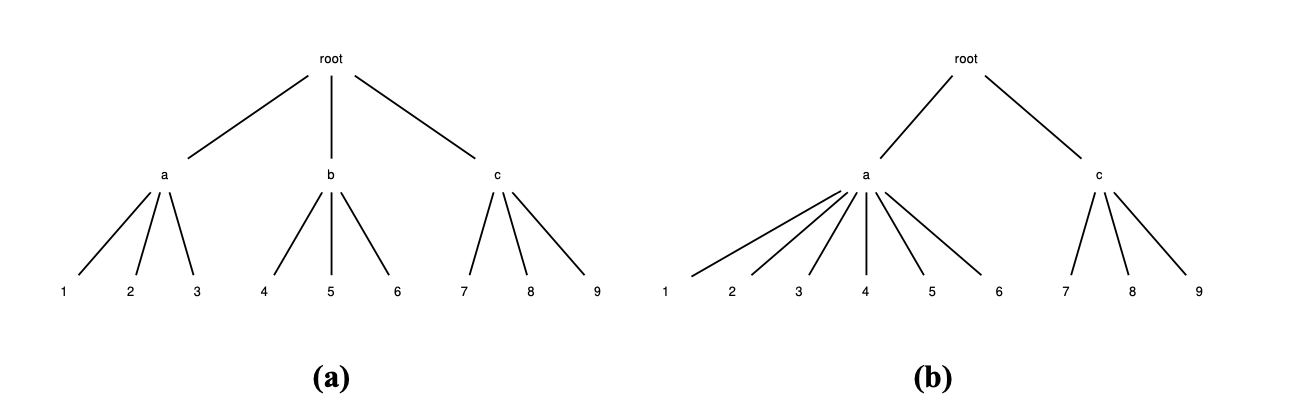
\includegraphics[width=.9\linewidth]{./asset/merging-operator.png}
\caption{\label{fig:merging-operator}融合算子}
\end{figure}

\item 联合算子
\label{sec:org28a6a52}
令 \(T\) 是一棵编码树, \(\alpha\) 和 \(\beta\) 是树中的兄弟节点且 \(\alpha^{-}=\beta^{-}=\delta \in T\) , 定义联 合算子 \(C b(T ; \alpha, \beta)\) 如下:

(1) 构造一个新的树节点 \(\xi\), 满足 \(T_{\xi}=T_{\alpha} \cup T_{\beta}\) 和 \(\xi^{-}=\delta\) 。

(2) 令以 \(\alpha\) 和 \(\beta\) 为根的两棵子树变成以 \(\xi\) 为根的两棵子树, 即 \(\alpha^{-}=\beta^{-}=\) \(\xi \in T\), 两棵子树保持在原编码树 \(T\) 中的结构。

(3) 赋值 \(h(\xi)=h(\alpha)=h(\beta), h(\alpha)=h(\beta)=h(\xi)+1\), 以 \(\alpha\) 和 \(\beta\) 为根的两棵子树中所有的树节点高度均增加 1 。
记 \(T^{\prime}=T_{c b}(\alpha, \beta)\) 为 \(C b(T ; \alpha, \beta)\) 运行之后的编码树, 容易求出编码树 \(T_{c b}(\alpha, \beta)\) 和 \(T\) 确定的图 \(G\) 的结构信息的差:

$$\begin{array}{r}
\Delta_{G}^{C b}(T ; \alpha, \beta)=H^{T}(G ; \alpha)+H^{T}(G ; \beta) \\
-\left(H^{T^{\prime}}(G ; \xi)+H^{T^{\prime}}(G ; \alpha)+H^{T^{\prime}}(G ; \beta)\right) .
\end{array}$$

如果 \(\Delta_{G}^{C b}(T ; \alpha, \beta)>0\), 那么联合算子运行成功, 记为 \(C b(T ; \alpha, \beta) \downarrow\) 。根据上式可知, \(\Delta_{G}^{C b}(T ; \alpha, \beta)\) 是局部可计算的。联合算子将两棵子树联合成一棵新 的子树, 赋予一个新的前驱节点。两棵子树中所有树节点的高度增加 1 , 编码树 中其他的节点没有变化, 如图\ref{fig:combining-operator}所示。

\begin{figure}[htbp]
\centering
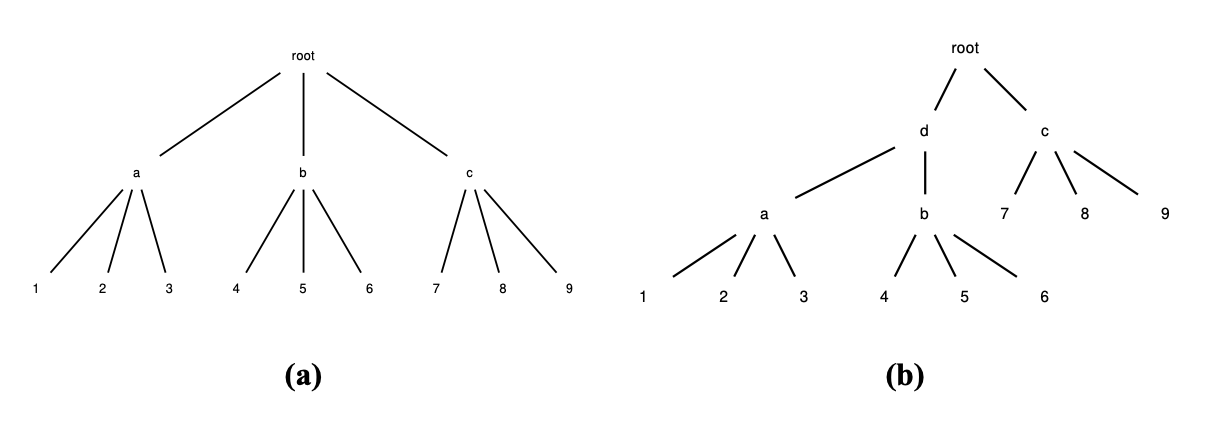
\includegraphics[width=.9\linewidth]{./asset/combining-operator.png}
\caption{\label{fig:combining-operator}联合算子}
\end{figure}
\end{enumerate}

\subsubsection{算法的时间复杂度}
\label{sec:org11f0fa5}
当 \(K=2\) 时, \(\mathcal{E}^{2}\) 的时间复杂度为 \(O\left(n^{2}\right)\), 当 \(G\) 是稀疏图时, 采用类似 \({ }^{[70]}\) 的 数据结构实现算法, 时间复杂度为 \(O\left(n \cdot \log ^{2} n\right)\), 其中 \(n\) 是图中顶点的数目。当 \(K=3\) 时, 对于编码树中每一个高度为 1 的节点 \(\alpha, T_{\alpha}\) 包含的顶点数目在算法运 行的过程中不会减小, 如果 \(\left|T_{\alpha}\right|=M\), 那么 \(M\) 满足 \(1 \leq M \leq n\) 。 对于一个固定 大小为 \(M\) 的 \(T_{\alpha}\), 算法在以 \(\alpha\) 为根的子树上运行的时间复杂度就是在顶点数目为 \(M\), 顶点集合为 \(T_{\alpha}\) 的 \(G\) 的子图上运行 \(\mathcal{E}^{2}\) 的时间复杂度, 为 \(O\left(M^{2}\right)\), 当 \(G\) 是稀 疏图时为 \(O\left(M \cdot \log ^{2} M\right)\) 。在编码树中高度为 1 的节点数目最多是 \(n\), 因此 \(\mathcal{E}^{3}\) 时 间复杂度为 \(O\left(n^{3}\right)\), 当 \(G\) 是稀疏图时为 \(O\left(n^{2} \log ^{2} n\right)\) 。虽然 \(\mathcal{E}^{K}\) 的时间复杂度是多项式的, 但是很难识别一个大规模网络的 \(K>3\) 维划分结构。因此, 本文只讨论 \(K=2\) 和 \(K=3\) 的情况。

\subsubsection{图结构熵和香农熵的比较}
\label{sec:orge21f1e2}
最后,在本章中将图结构熵和香农熵进行比较,分析两者的异同。结构熵度 量嵌入在图中的信息(不确定),其定义受香农熵的启发,但是在以下几个方面 和香农熵有所不同:

\begin{itemize}
\item 这两个熵定义在不同的领域中。结构熵定义在有结构的图上,而香农熵定 义在无结构的概率分布上。因此,结构熵度量了嵌入在图中的信息,而香农熵度 量了一个概率分布的信息。
\item 结构熵直接和图结构相关联,与编码树有关,而香农熵没有结构相关联, 与编码树无关。给定一个图 G 和 G 的一个编码树 T ,T 对应 G 的一个层次划分 结构, \(H^T (G)\) 是在这个层次划分结构中进行随机游走的不确定性。当限制 T 的 高度为 K 时,得到 K 维结构熵,特别地,当 T 的高度为 1 时,\(H^1(G)\) 退化为 G 的度分布的香农熵。换句话说,可以计算 G 的任意层次划分的结构信息,然而, 对于任意的概率分布,香农熵仅仅是一个度量该分布不确定性的一个数字。
\item 结构熵度量一个图的动态信息量,而香农熵定义在无结构的概率分布上, 因此只是一个概率分布的静态信息量的度量。
\item 结构信息解码出图的一个实质结构,该实质结构支撑图的语义分析。而香 农熵不支持语义分析,仅仅提供一个全局不确定的度量。
\end{itemize}

总结起来,结构熵针对有结构的图,解码出实质结构,进而支撑语义和功能 分析。香农熵研究概率分布,得出统计结论,不支持数据的精确分析,不足以建 立数据分析的解释原理,而结构信息支持数据的精确分析,并能够建立数据分析 的可解释原理。


\section{图结构熵解码低分辨率 Hi-C 数据的染色质拓扑结构域}
\label{sec:orgbd78221}
在哺乳动物细胞中,几米长的基因组通过折叠形成复杂的三维结构存在于 几微米大小的细胞核中,如图\ref{fig:chromatin-spatial-structure}所示,而基因组的三维结构则决定着细胞核中

\begin{figure}[htbp]
\centering
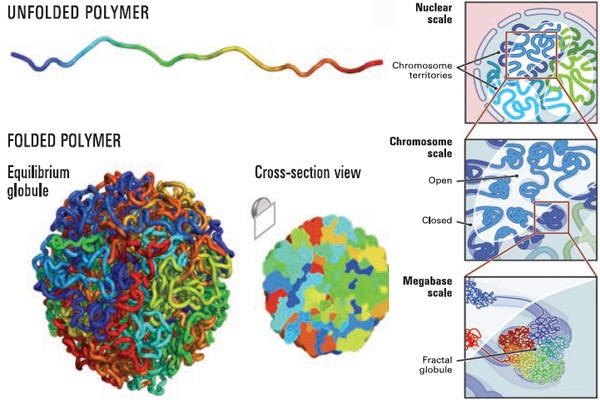
\includegraphics[width=.9\linewidth]{./asset/chromatin-spatial-structure.jpg}
\caption{\label{fig:chromatin-spatial-structure}染色质空间结构}
\end{figure}

的许多生命过程。在过去的十年里,染色体构象捕捉技术和其变体在阐释 染色体结构上的成功极大地刺激了对基因组三维结构的探索,随着数据地不 断积累,尤其是高通量染色质相互作用\citep{lieberman2009comprehensive}(简称 Hi-C)数据的应用,基因组的拓 扑结构开始显现。Hi-C 实验的具体过程如图\ref{fig:hic-experiments}所示,其主要包含如下几步:

\begin{figure}[htbp]
\centering
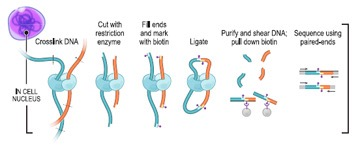
\includegraphics[width=.9\linewidth]{./asset/hic-experiments.jpg}
\caption{\label{fig:hic-experiments}Hi-C实验步骤}
\end{figure}

\begin{enumerate}
\item 用甲醛固定染色质,染色质由双链 DNA 构成。
\item 用限制性内切酶切开染色质。
\item 用核苷酸填充切开的端点,生物素标记切开的位置。
\item 把两条染色质的端点结扎起来,端点越近,结扎成功概率越高。
\item 结扎成功后,切开生物素标记位置。
\item 对生物素标记过的配对末端进行两端测序。
\item 将测序结果比对到全基因组上,得到基因位点对的一个测序读数。
\end{enumerate}

最后,将得到的测序数据再做一些信噪处理\citep{lieberman2009comprehensive},得到最终的 Hi-C 数据。Hi-C 实验通常在上百万个细胞上进行,最终得到染色质位点对之间的测序
读数,将位点对对应于矩阵中的行列坐标,然后得到一个对称矩阵,称为 Hi-C矩阵,如果位点对之间有测序读数,那么矩阵中相应的行列值为 1。几米长的染 色质位点数目多达几亿,那么矩阵包含几亿行几亿列,处理该矩阵显然非常困 难,通常将染色质中特定的长度(称为 binsize)收缩成一点(称为 bin),该点对 应矩阵中行或列的坐标。然后对原矩阵进行收缩,得到可计算的 Hi-C 矩阵,矩 阵中行列的值为该行列 bin 在原矩阵中对应的子矩阵所有值的和。图\ref{fig:hic-heatmap}是人体 胚胎干细胞第 21 条染色体测序结果对应的 Hi-C 矩阵,binsize 为 40kb,染色体 长度大约为 44mb,颜色深浅表示相应 bin 之间测序读数的多少。在染色质空间 结构中,位置越近的片段彼此之间的测序读数越多,对应在 Hi-C 矩阵中相应的 对角线区域颜色越深,形成一块深色矩形区域,那么组成该区域的 bin 集合就越 有可能是空间中纠缠在一起的一段结构域。相邻的结构域之间的区域称为边界 区域。只有当用于测序的细胞和测序读数足够多时,矩阵中对角线的深色矩形区 域才能显现出来,进而显现出结构域。

\begin{figure}[htbp]
\centering
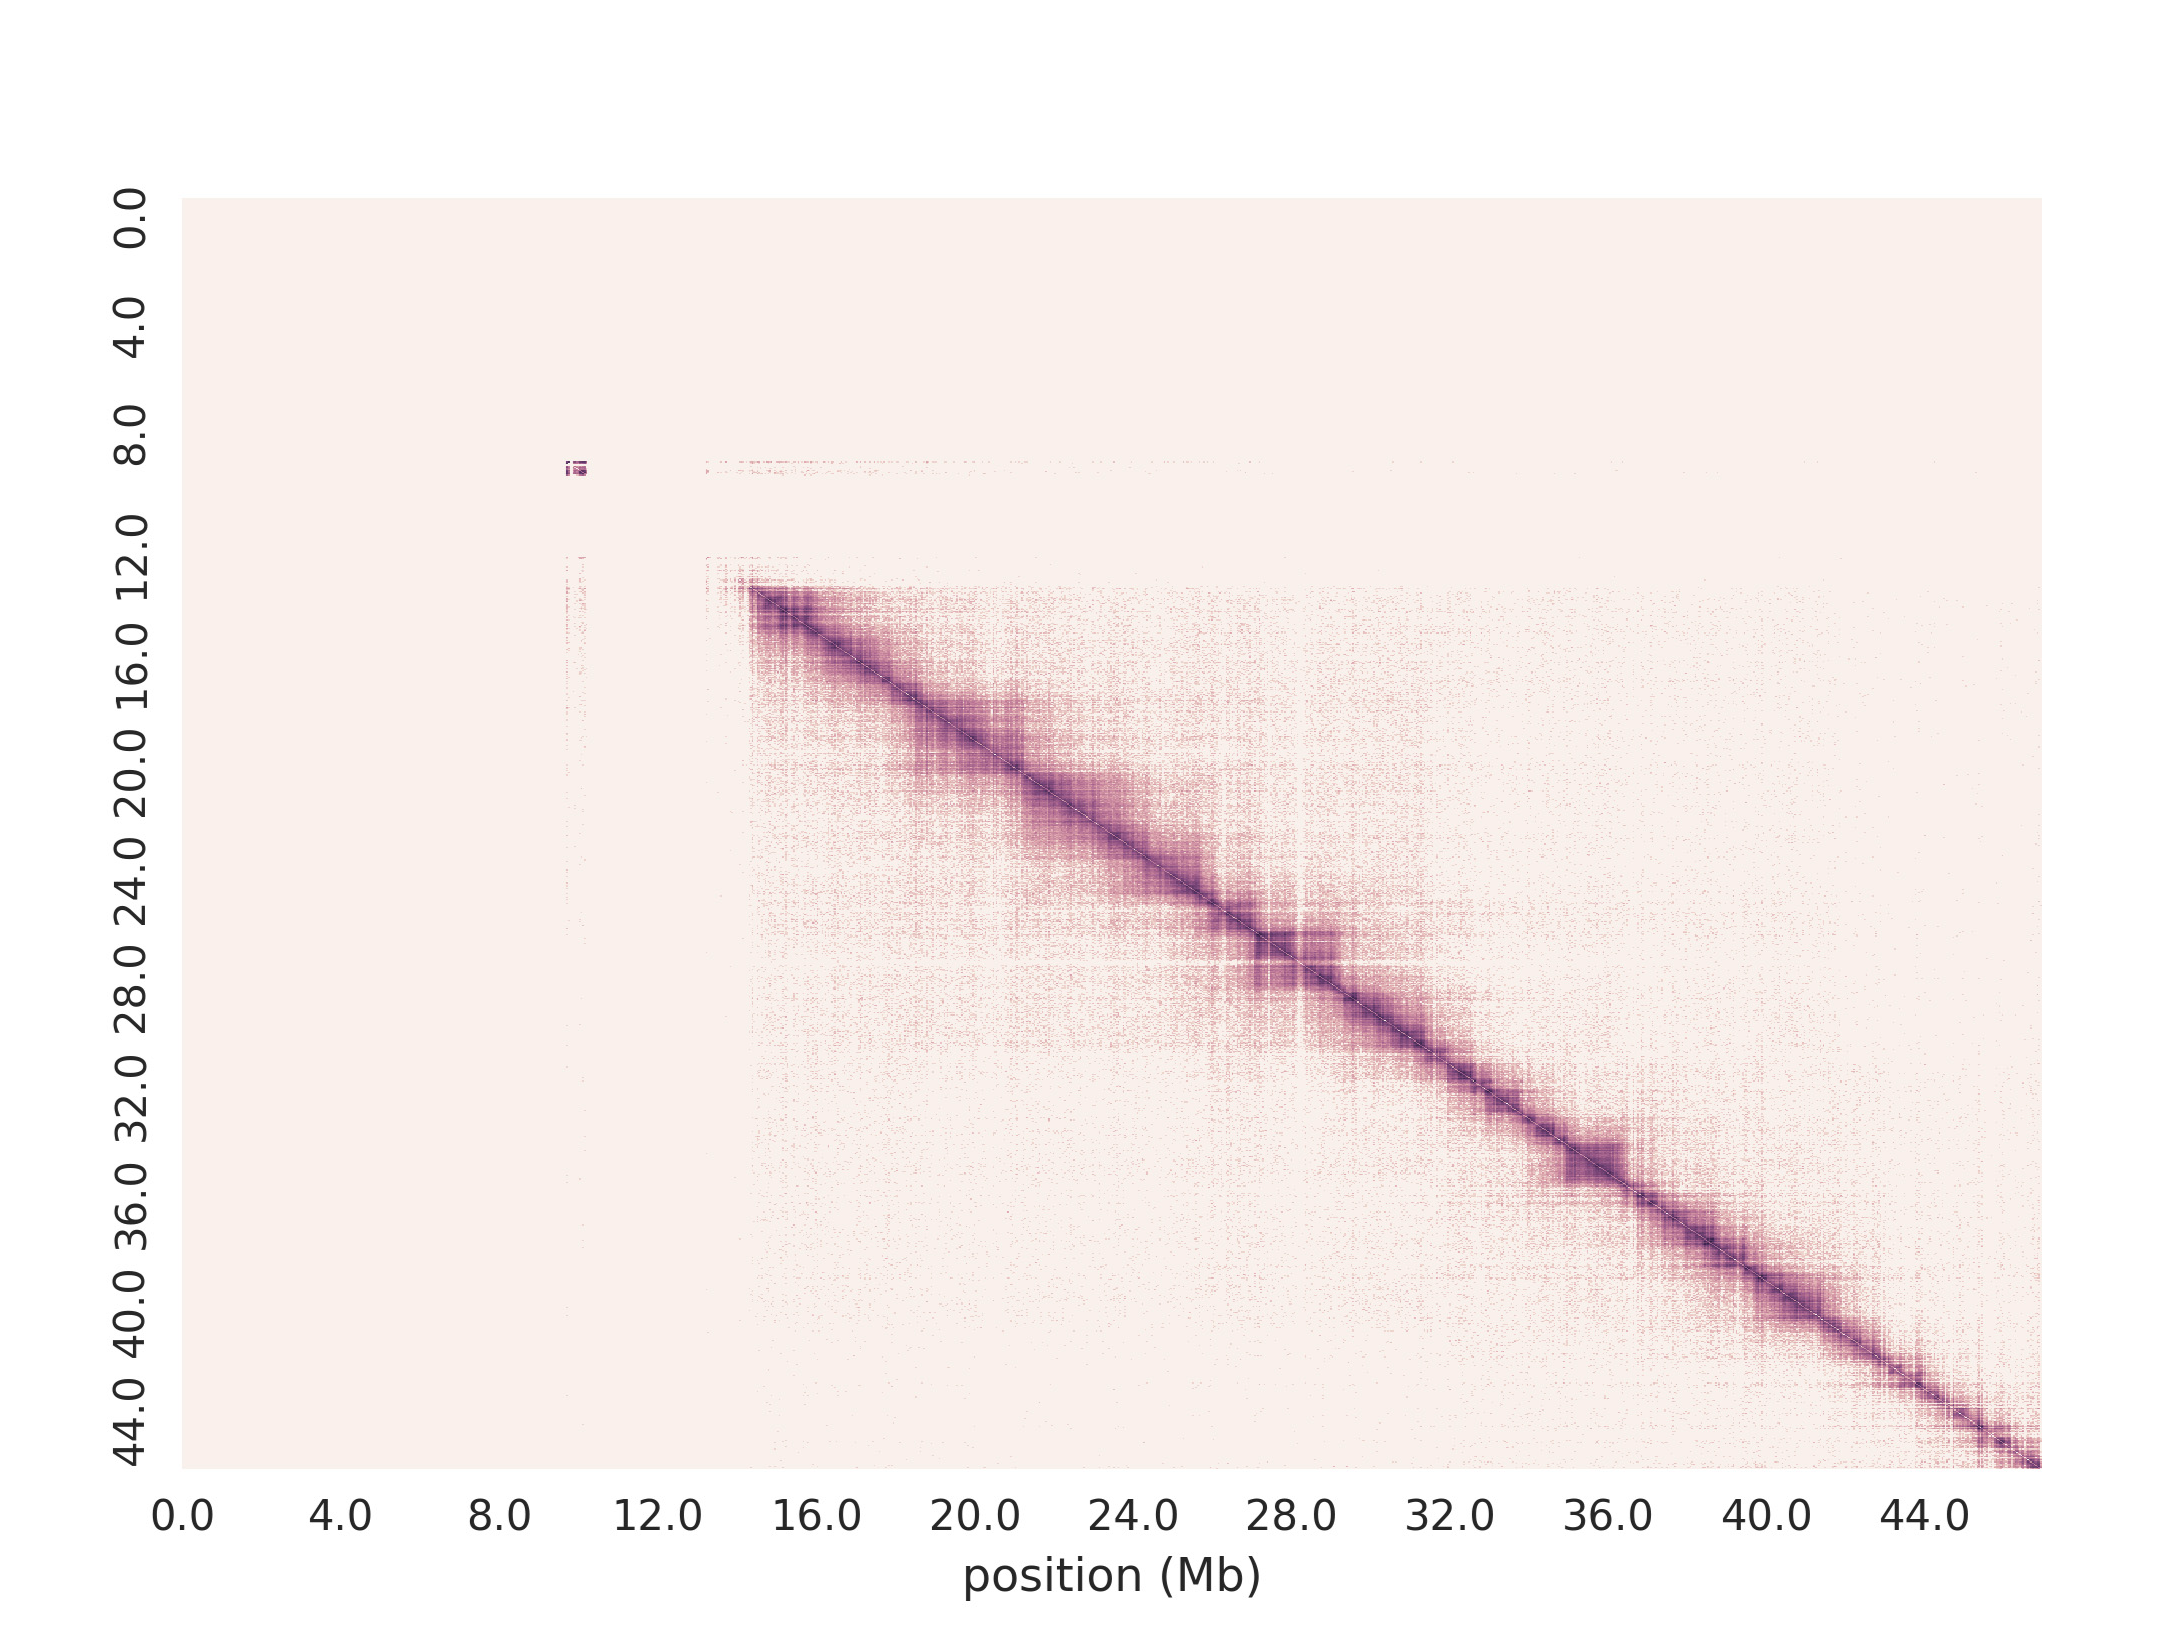
\includegraphics[width=.9\linewidth]{./asset/hic-heatmap.png}
\caption{\label{fig:hic-heatmap}人体胚胎干细胞第21条染色体的Hi-C矩阵热力图}
\end{figure}

每条染色体都可以大致划分为活跃的区隔和不活跃的区隔,这些区隔可以进一步分为结构域,通常在哺乳动物中称为拓扑结构域。拓扑结构域被发现带有基因调控中靶向启动子的增强子,并且和复制调控区域的相关性强,并在不同细胞类型和物种中保守。而且拓扑结构域边界的破坏可能导致癌症等疾病的发生,因此对拓扑结构域的预测研究在文献中备受关注。

一些预测拓扑结构域的算法已经被开发出来。Dixon 等\citep{dixon2012topological}首次 给出了预测结构拓扑域的方法,称为 Domaincall,该方法基于隐马尔可夫模型,通 过检测出染色质相互作用有偏差的上游和下游区域来预测拓扑结构域。Filippova 等\citep{filippova2014identification}引入了分辨率特定域的概念,利用动态规划算法预测拓扑结构域,该方 法称为 Armatus。

即使上述方法取得了成功,但是关于拓扑结构域及其预测的几个基本问题 仍然具有挑战性。首先,决定基因组层次结构的全局约束仍有待阐明。这个问 题可以通过在预测拓扑结构域 时设置一个全局目标函数来解决,但是这 些目标函数都是拓扑度量,如基因组距离和基因组的模块度,所以至今 仍无法知道是什么全局约束定义了基因组的层次拓扑结构域。第二,确定一个 给定 Hi-C 数据集的恰当 binsize 的方法尚未形成。由于染色质交互数据的稀疏性 和噪声性,需要将 Hi-C 数据分成长度适合的 bin 来进行下一步分析,bin 的长度 binsize 是 Hi-C 数据分析的关键,不恰当的 binsize 设置可能会导致不正确的结果 或者造成测序数据的浪费。然而,在当前的实践中,binsize 大部分都是任意定 义的。第三,如何用低分辨率(极其稀疏)的 Hi-C 数据可靠、稳定地预测拓扑 结构域的问题还没有得到解决。目前几乎所有的算法都需要超高的数据分辨率 来识别基因组拓扑域结构,然而随着 Hi-C 技术的应用范围不断扩大,对更深测 序深度的要求已经成为进一步发展越来越大的障碍,尤其是单细胞环境中的应 用。最后,拓扑结构域最初是在大样本细胞中观察到的 Hi-C 数据的一种统计特 性。大样本中可能包含数百万个细胞,而单细胞 Hi-C 数据显示基因组 结构具有高度的动态性,它随着细胞间基因组空间结构的变化而变化。尽管汇集 了数千个单个细胞的 Hi-C 数据确实重构了拓扑结构域的集合,但是拓扑结 构域(或者使用更通用的术语“模块化结构”)对于一个小细胞群体来说到底有多 本质还是一个有待解决的问题。

有人基于结构信息开发一个名为 deDoc 的染色质拓扑结构域预测方 法来解决上述问题。结构信息(或熵)度量了嵌入在图中的动态不确定性,最小化结构熵(简称 SE)是对图的本质结构进行解码的一种直观方法,它将由随机变 化和噪声引起的扰动产生的影响降到最小。deDoc 将 Hi-C 联系矩阵作为图的邻 接矩阵,构造 Hi-C 图,基于结构熵极小化原理识别具有极大确定性的三维基因 组结构。 deDoc 区别于其他最先进方法有五个突出特点。首先,该方 法基于结构信息论。与大多数主要基于局部联系结构的最先进方法不同,deDoc 是一种图方法,它旨在抽取出一个最小化 Hi-C 图全局不确定性的结构。其次, deDoc 可以很好地处理原始 Hi-C 数据,不需要对原始数据进行任何正规化操作, 而且 deDoc 无需手动选择参数。这就排除了在正规化或手动选择参数时引入噪 声的影响。第三,deDoc 适用于高度稀疏的 Hi-C 图,这意味着 deDoc 对输入数 据的数据量具有很强的鲁棒性。第四, deDoc 可以用于定量确定给 定 Hi-C 数据集的最佳 binsize。

\section{基于结构信息的文本聚类}
\label{sec:org8420d84}
聚类问题是计算机科学和信息科学中一个基本问题。聚类的本质就是将相 似的对象集合聚成一类,而文本聚类是聚类问题中最经典的问题之一。给定一个 没有主题的文本集合,文本聚类将具有相同主题的文本集合组织在一起,以便于 以后的查阅及搜索。好的文本聚类方法可以辅助计算机自动将语料库中的文本 组织成具有相同主题的类别,从而能够更有效地浏览语料库,更容易地理解语料 库的内容。因此,研究人员提出了很多方法用于文本聚类。

绝大多数文本聚类方法的第一步是构建文本表示的向量空间模型,将文 本中的词项看作特征,文本表示成特征空间的向量,文本向量之间的相似度计 算通常采用余弦相似度。凝聚式层次聚类初始时将每一篇文本看作一个 类别,然后迭代合并最相似的两个类别直到终止条件满足。k 均值聚类是应用最 广泛的聚类方法之一,Dhillon 等\citep{dhillon2001efficient}将 k 均值聚类应用在了文本聚类中,首 先对向量空间中的文本向量进行归一化操作,使得文本向量落在单位半径的球 面上,然后初始化 k 个中心向量,采用余弦相似度计算文本向量与类别中心向 量之间的距离,最后将每一个向量赋给最近的中心所代表的类别,在下一次迭 代中,新的文本类别中心向量则定义为该类别中所有文本向量的和并进行归一 化,一直迭代直到满足终止条件。除了单方面聚类文本的方法之外,还有很多方 法同时聚类文本和词项,输出文本和词项的类别,统称该类方法为共同聚类。图 划分算法是其中应用最广泛的方法,该方法首先将文本和词项的关系表示成二部图,文本和词项各为一类顶点,文本与其包含的词项有边相连,然后根 据不同的图划分目标函数进行优化,最后同时得到文本类别及与该类别有相同 主题的词项类别。应用在文本聚类领域的图划分目标函数主要有关联率、割 率、K-L 目标和正规化割等。Dhillon 等\citep{dhillon2003information}提出了基于信息论的 方法,将文本和词项看作离散型随机变量,将文本词项频率矩阵当作两个随机 变量的经验联合概率分布,通过最小化共同聚类前后的经验概率分布的互信息 损失,来得到高质量的文本类别和词项类别。Xu\citep{xu2003document}等 提出了非负矩阵分解的 方法,将文本词项矩阵分解成两个非负矩阵,分别对应文本类别矩阵和词项类 别矩阵,并证明了非负矩阵分解的方法显著优于隐形语义索引的方法。Long 等\citep{long2005co}提出了矩阵块值分解的方法,将文本词项矩阵分解成三个矩阵,包括行系 数矩阵、列系数矩阵和块值矩阵,块值矩阵中的值代表文本类别和词项类别之间 的关系,并证明了非负矩阵分解是矩阵块值分解的特例。

可以基于结构熵极小化原理给出一个文本聚类的新方法。首先基于文本 词项矩阵构造了文本与文本之间的近邻图,根据一维结构熵极小化原理选择近 邻图中每个顶点的边数。其次,基于二维和三维结构熵极小化原理对文本近邻图 进行划分,划分结果就是文本聚类的类别,同时构造文本词项表示谱图。然后, 在标准数据集上和已有文本聚类算法进行比较,效果要优于其他算法。最后,将 每类文本的代表性词项整理出来,根据词项可以推断出每类文本的类别主题。

\section{基于结构信息的局部列举排名}
\label{sec:org2845766}
网络中的搜索是识别查询节点或查询集的自然社区。当前的搜索引擎是在 Brin 和 Page 引入 PageRank 的基础上开发出来的,这种思想为当前的搜索 引擎提供了基础。PageRank 理论表明如果一个页面被其他重要页面指向,那么 该页面就重要。基于 PageRank 理论,可以建立 PageRank 方程,利用幂法求出 唯一的 PageRank 向量,该向量则定义了图中各个顶点的排名。搜索引擎中使用 的 PageRank 向量在计算过程中引入了具有均匀分布的偏好向量,即从当前 顶点以相同的概率跳转到所有顶点中以保证得到唯一的 PageRank 向量。Haveliwala 提出了将偏好向量中的概率分布集中到特定的顶点集合中,以得到个性化 PageRank 向量的方法。Jeh 和 Widom 以及 Fogaras 和 Racz 对个性化 PageRank 向量进行了扩充。Guha 等\citep{guha2004propagation}提出了具有正负权重的图的 PageRank 值。

虽然基于 PageRank 的搜索引擎已经得到了广泛应用,但是仍然有一些基本 问题有待回答,比如:基于 PageRank 的搜索引擎到底有多好?搜索引擎的背后 原理到底是什么?未来的搜索引擎能否给查询一个专家的回答?为了回答这些问 题,必须要理解在自然界和社会中演化的网络,其自然社区结构形成的机制和原理是什么。

网络最开始被假定为随机演化的。Erdös 和 Rényi 提出了一个经典的网 络随机演化模型,称为 ER 模型,该模型研究了随机图的许多特征,包括大连通 分支和小直径等特征。此外,Watts 和 Strogatz 提出了一个向网格图中添加随 机边的简单模型。类似地,Kleinberg 引入了向网格图的端点之间添加边的模 型,其添加边的概率反比于端点之间距离的幂。这些模型生成的图具有小世界 现象,并且具有聚类效应,即如果两个顶点有共同的邻居,那么它们更有可能 是相连的。Barabási 等通过引入偏好依附作为显示的机制提出了无标度模型, 生成了度分布是幂律分布的图。在此基础上,利用随机性和一些局部规则引入 了许多新的模型,包括复制模型、森林火模型、随机游走和最近邻模 型、随机冲浪模型和分层模型,这些模型为统计鲁棒性提供了理论方 法。此外,还有一些具有特定社区结构的模型,例如 l 划分种植模型和 LFR 模型,可以通过调整模型的参数生成具有不同社区结构的网络。

Li 等\citep{li2015discovering}提出了一种基于网络适应度的社区发现算法。将该算法应用在一些 真实世界的网络中,结果表明在算法发现的真实世界的网络群体中,大多数个体 具有共同的属性,因此同源性是网络预测的原则。该结果也暗示了同源性是亲缘 关系在高层网络中的延伸,而同源性/亲缘性关系是真实网络中随机变化的控制 原理。此外,Li 等\citep{li2015discovering}提出了同源性/亲缘性模型,通过引入亲缘性指数的概念来 捕获自然界和社会中自然演化的网络。这些结果首次探索了真实世界网络与达尔文进化论中的物种之间的相似性,而同源性是真实世界网络自然社区形成 的内在机制和原理。

可以基于结构信息,实现了局部列举排名算法,从初始查询点出发,判 断算法是否能够将该点所在的真实社区输出为查询结果集合。算法应用到包含 社区结构的同源性/亲缘性模型、l 划分种植模型 和 LFR 模型,效果明显好于基于谷歌 PageRank 的局部搜索算法。该结果为搜索引擎的搜索算法提供了一个新的思路。

\section{总结与展望}
结构信息论是刻画图结构信息的基本理论,通过图结构的编码树来解码图中的结构信息。基于结构信息论,我们提出了数据分析的如下原理:
\begin{itemize}
    \item 一维结构熵最小化是非结构数据结构化的原理。
    \item 二维、三维、高维结构熵极小化是大数据空间结构信息解码的原理。
    \item 大数据空间有一个功能语义,它由一个实质结构支撑,该实质结构通过结构信息解码求解。
\end{itemize}

我们通过分析高通量染色质相互作用、文本数据和模型网络数据,验证了基于结构信息的数据分析原理。我们通过应用数据分析原理的算法,首先将非结构化数据结构化,然后解码出了图的划分结构,最后分析出了划分结构的语义。

结构信息论是一个全新的原始创新的理论,解决了建立结构的信息理论这一难题。而基于结构信息进行数据分析还处于起步阶段,目前找图的最优编码树的算法仍然是简单的贪心算法,仍有很大的改进空间。随着大数据时代的到来,数据量不断增长,设计合适的结构熵极小化算法以适应处理大数据的需求也变得非常重要。

\section{参考文献}
\label{sec:org9101910}
\bibliographystyle{apacite}
\bibliography{materials/library}
\end{document}
